\documentclass[14pt]{report}
\usepackage{geometry}                % See geometry.pdf to learn the layout options. There are lots.
\geometry{letterpaper}                   % ... or a4paper or a5paper or ... 
%\geometry{landscape}                % Activate for for rotated page geometry
%\usepackage[parfill]{parskip}    % Activate to begin paragraphs with an empty line rather than an indent
\usepackage{graphicx}
\usepackage{amssymb}
\usepackage{epstopdf}
\DeclareGraphicsRule{.tif}{png}{.png}{`convert #1 `dirname #1`/`basename #1 .tif`.png}

\title{MLPR Assignment}
\author{I.D s0840844}
%\date{}                                           % Activate to display a given date or no date
\DeclareMathSizes{10}{10}{9}{8}
\begin{document}
\begin{flushleft}
\maketitle
%\section{}
%\subsection{}
\section { Bayesian Analysis of Uniform distribution}

Given  
$ p(\theta) \sim Pa(b,K) $= \left\{ \begin{array}{rcl} \frac{Kb^k}{\theta^{K+1}}   & \mbox{for } \theta \geq b  \\ 0 & \mbox{otherwise} \end{array}\right


Now with the above Pareto prior, the joint distribution of $\theta$ and $D =\{ x_1,x_2,....x_N\}$ is:
\[ p(D,\theta) =P(D|\theta)P(\theta) = \left\{ \begin{array}{rcl} \frac{1}{\theta^N} . \frac{Kb^K}{\theta^{K+1}} &\mbox { for }  \theta \geq max(max(D),b) \\0 & \mbox{otherwise} \end{array}\right

With the given definition of $P(D)$ and taking $m=max(D)$ , the posterior  $p(\theta|D)$ can now be defined as follows:
\begin{flushright}
\begin{eqnarray*}
 p(\theta|D) = \frac{P(\theta,D)}{P(D)}&=&  \left\{  \begin{array}{rcl}\frac{\frac{1}{\theta^N} . \frac{Kb^K}{\theta^{K+1}}}{\frac{K}{(N+K)b^N}} & \mbox{for  } b\geq m \mbox{ and } b\leq \theta \\ \frac{\frac{1}{\theta^N} . \frac{Kb^K}{\theta^{K+1}}}{\frac{Kb^K}{(N+K)m^{N+K}}} & \mbox{for  } m > b \mbox{ and } m\leq \theta \end{array}\right \\ 0 \mbox{ otherwise}\\
 \end{eqnarray}
 \end{flushright}
 This can be simplified and written as: 
 \begin{flushright}
 \begin{eqnarray*}
 p(\theta|D) = \frac{P(\theta,D)}{P(D)}&=& \left\{ \begin {array}{rcl} \frac{(N+K)b^{N+K}}{\theta^{N+K+1}} \mbox{ for }  b\geq m \mbox{ and } b\leq \theta\\
  \frac{(N+K)m^{N+K}}{\theta^{N+K+1}} \mbox{ for }  m > b \mbox{ and } m\leq \theta \\    \end{array}\right
\end{flushright}  
 
\end{eqnarray}
Note : For b $\geq$ m , $p(\theta|D)$ =0 for $\theta < b$ and similarly for $ m > b$ $   p(\theta|D) =0 $ for $\theta < m$.

The posterior in fact has the same function functional form as a Pareto distribution :
 
 We know the Pareto distribution, Pa is defined as : $ Pa(\alpha, n) =  \frac{\alpha n^\alpha}{\theta^{\alpha+1}}$. If we compare this with the above distribution, we can see $\alpha \equiv  (N+K)$ and $n \equiv \{ m,b\}$

\section{The Tramcar problem}
\subsection{Part A}

Assumptions made: 
\begin{itemize}
\item trams are numbered sequentially as integers starting from 0 to some upper bound $\theta$. Thus the likelihood function $p(x)$ can be defined as:

\[ p(x) = f (x|\theta) = \left\{ \begin{array}{rcl} \frac{1}{\theta} \mbox { for } 0 \leq x \leq \theta \\ 0  \mbox{ otherwise} \end{array}\right\]

\item K=1 and b=1 and the D=\{100\} .
This implies m= 100 
\end{itemize}
Since $ m>b$ the posterior $p(\theta|D)$ is given as :
\[ p(\theta|D) =   \frac{(N+K)m^{N+K}}{\theta^{N+K+1}} = \frac{2. 100^2}{\theta^3} \]

\subsection{Part B}
The posterior $p(\theta|D)$ as shown above is a Pareto distribution. Hence the mean and maximum posterior of   $p(\theta|D)$ can derived using the properties of a Pareto distribution.

\[ \mu (mean) =\frac{(N+K)m}{N+K-1} = \frac{2m}{1} = 200\]
\[ MAP = mode = m = 100\]

\subsection{Part C}
The predictive  density  is given by $p(x|D) = \int_{0}^{\infty} p(x|\theta)p(\theta|D)d\theta$.

As already stated in part A , $p(\theta|D)=0$ for $\theta <m$ thus 
\begin {eqnarray*}
 p(x|D) & =& \int_{m}^{\infty} p(x|\theta)p(\theta|D)d\theta\\
 p(x|D) &	       =&   \int_{100}^{\infty} \frac {1}{\theta} . \frac{2. 100^2}{\theta^3} d\theta \\
                     &=& [ \frac{-2.100^2}{3.\theta^3}]_{100}^{\infty}\\
                     &=& \frac {2}{3.100} \\
                     &=& \frac{1}{150}
\end{eqnarray}

\subsection{Part D}
 From Part C, it is clear that the predictive distribution $p(x|D)$ is a uniform distribution $U(x,\theta)$  where $\theta= 150$:
  
\[ p(x|D)  = \left\{ \begin{array}{rcl} \frac{1}{150} \mbox { for } 0 \leq x \leq 150 \\ 0  \mbox{ otherwise} \end{array}\right\]

Therefore for a new data point \textbf{x}, the prediction is :
\[ p(\textbf{x} | D) = \frac{1}{150} \large{I}(\textbf{x} \in [0,150]) =  \frac{1}{150} \large{I}(\textbf{x} \leq150)\]

For observations whose value lie outside 150, the probability of observing them given the dataset D is 0.
Thus $p(50|D)$ =$\frac{1}{150}$ and $p(500|D)$ =0.

\subsection{Part E}
As K \longrightarrow 0 

$\lim_{ K \rightarrow 0}p(\theta)  =0$. Thus the limit of  posterior $p(\theta|D) $ when K tends to 0  :

\[ \lim_{ K \rightarrow 0} p(\theta|D)= \frac{P(\theta,D)}{P(D)}&=& \left\{ \begin {array}{rcl} \frac{(N)b^{N}}{\theta^{N+1}} \mbox{ for }  b\geq m \mbox{ and } b\leq \theta\\
  \frac{(N)m^{N}}{\theta^{N+1}} \mbox{ for }  m > b \mbox{ and } m\leq \theta \\    \end{array}\right

Observations:
\begin{itemize}
\item As $K \rightarrow 0$,  the posterior $p(\theta|D)$ at the limiting value of K is still a Pareto distribution.  Sending K to 0 tends to change only the shape parameter of the original posterior distribution which is illustrated as follows:

We know $ Pa(\kappa, n) =  \frac{\kappa n^\alpha}{\theta^{\kappa+1}}$.

By comparing the above distribution with our original posterior $p(\theta|D)$, we concluded that $ \kappa \equiv (N+K) $ but as K\rightarrow 0    $ \kappa \equiv N$  



By observing the graph below, we can see that decreasing the value of the shape parameter $\kappa$ makes the distribution more heavily tailed.  Thus, rare instances will have a greater probability mass assigned to them than before.  Having the posterior  $p(\theta|D)$  more heavily tailed  improves the predictive density that we computed in Part C.


\[\lim_{k\rightarrow 0} p(x|D) =   \int_{100}^{\infty} \frac {1}{\theta} . \frac{1. 100^1}{\theta^2} d\theta = \frac{1}{200}\]
Therefore for a new data point \textbf{x}, the prediction is :
\[ p(\textbf{x} | D) = \frac{1}{200} \large{I}(\textbf{x} \in [0,200]) =  \frac{1}{200} \large{I}(\textbf{x} \leq200)\]
Although the individual probability of observing each individual tram within the range [0-150] is less than before, by assigning probability masses on trams between 150 and 200, the predictor improves prediction by increasing the set of trams that it believes that we might see next. In other words the predictor moves towards the true uniform distribution.


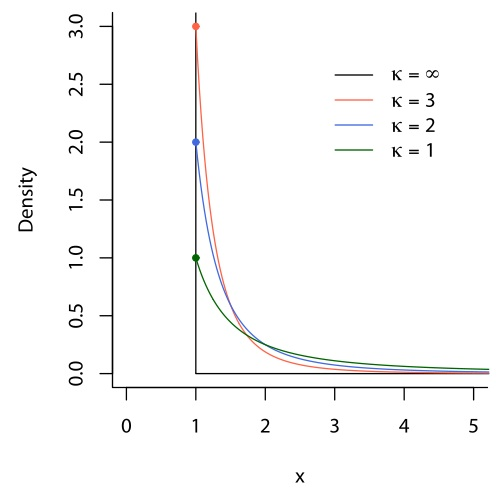
\includegraphics[ scale=0.5]{Pareto.jpg}



\end{itemize}

\end{flushleft}

\end{document}  